\documentclass[11pt,twoside,a4paper]{book}

\usepackage[czech, english]{babel}
 \usepackage[OT1]{fontenc} % pouzije EC fonty
\usepackage[utf8]{inputenc}
\usepackage{lmodern}
\usepackage{graphicx}

\usepackage{mathtools}
\usepackage{indentfirst} %1. odstavec jako v cestine.
\usepackage{k336_thesis_macros} 
\usepackage{hyperref}
\hypersetup{
    bookmarks=true,         % show bookmarks bar?
    unicode=true,			% non-Latin characters in Acrobat’s bookmark
    colorlinks=true,       	% false: boxed links; true: colored links
    linkcolor=blue,			% color of internal links (change box color with linkbordercolor)
    citecolor=blue,        	% color of links to bibliography
}

\usepackage[square, numbers]{natbib}             % sazba pouzite literatury


\newcommand\Department{Katedra počítačů}
\newcommand\Faculty{Fakulta elektrotechnická}
\newcommand\University{České vysoké učení technické v Praze}
\newcommand\labelSupervisor{Vedoucí práce}
\newcommand\labelStudProgram{Studijní program}
\newcommand\labelStudBranch{Obor}

\newcommand\TypeOfWork{Diplomová práce} \typeout{Diplomova prace}
\newcommand\StudProgram{Otevřená informatika, Magisterský}
\newcommand\StudBranch{Softwarové inženýrství}

\newcommand\WorkTitle{Pohledově závislá aplikace textur v reálném čase}
\newcommand\FirstandFamilyName{Bc. Daniel Princ} \newcommand\Supervisor{Ing.
David Sedláček, Ph.D.}


\let\oldUrl\url \renewcommand\url[1]{<\texttt{\oldUrl{#1}}>}


\begin{document}
\selectlanguage{czech} 

\coverpagestarts

\acknowledgements \noindent \noindent Chtěl bych poděkovat vedoucímu této práce,
panu Ing. Davidovi Sedláčkovi, Ph.D., za poskytnutí cenných rad a nápadů.

\declaration{V~Praze,  12. 5. 2014}
 
\abstractpage
TBD

\vglue60mm

\tableofcontents

\listoffigures

\listoftables

\mainbodystarts
% horizontalní mezera mezi dvema odstavci \parskip=5pt 11.12.2008 parskip +
% tolerance
\normalfont \parskip=0.2\baselineskip plus 0.2\baselineskip minus
0.1\baselineskip


\chapter{Úvod}
V dnešní době umožňuje počítačová grafika renderovat realistické obrazy 3D
světa. Nicméně aby toto bylo možné, musí existovat 3D modely objektů, které
chceme zobrazovat. Tradiční způsob, jak získat tyto modely, je jejich ruční
vytváření v modelovacích programech. To je velmi pracný a zdlouhavý proces
a~jeho výsledek není dostatečně realistický. Proto se v současnosti vyvíjí
postupy, jak přímo digitalizovat reálné objekty. Existují dva základní přístupy,
které se o toto pokoušejí. Nejpřesnější metoda je pravděpodobně laserové
skenování objektů. Druhou, mnohem levnější a dostupnější variantou, je rekonstrukce objektů z
fotografií. Těmito problémy se zabývá počítačové vidění a částečně také
počítačová grafika, do které spadá zobrazování rekonstruovaných modelů. Cílem 3D
počítačové rekonstrukce je tedy co nejvěrněji převést reálné objekty do
digitální podoby. Aplikaci najdeme ve virtuální realitě, online prohlídkách,
počítačových animacích nebo v herním či filmovém průmyslu.

Tato práce se zabývá jednou částí 3D rekonstrukce a to texturování objektů z
fotografií. Na vstupu očekáváme již zrekonstruovaný 3D model (síť trojúhelníků)
a větší množství (desítky až stovky) kalibrovaných fotografií z různých úhlů. Textura společně s materiálem slouží k popisu povrchu a je důležitá pro vnímání barvy a detailní struktury povrchu \cite{mpg}. Aplikace textury vede z výraznému zvýšení vizuální kvality objektu za relativně malou cenu.  Často je vizuálně i výkonově jednodušší použít detailní texturu a jednoduchý model s menším počtem vrcholů.

Syntéza textur z fotografií je poměrně složitá, protože 	na výsledný model se díváme i z jiných pohledů, než ze kterých byly pořízeny fotografie. Problémy, které při tomto procesu vznikají jsou popsány zejména v následující kapitole. Cílem této práce je vytvořit aplikaci, která v reálném čase mapuje fotografie na model. Protože aplikace funguje v reálném čase, může zohlednit aktuální pohled virtuální kamery a na základě pozice kamery vybrat nejvhodnější fotografie pro vytvoření textury. K tomu využívá velkého výkonu současných GPU.

[[obrázek model s a bez textur TODO]]


\chapter{Analýza problému a návrh řešení} %??

\section{Popis problému}

Předpokládejme, že se díváme na statickou scénu s konstantním osvětlením, kde se pohybuje pouze pozorovatel. Za těchto podmínek můžeme popsat libovolnou fotografii pomocí pozice a orientace kamery. Pokud bychom vyfotili sférickou fotografii v každé možné pozici kamery, mohli bychom vyrenderovat kompletní scénu z libovolného pohledu. Kombinací všech 3D pozic kamery $(x, y, z)$ a směrů $(\theta, \phi)$ získáme plenoptickou funkci $\textbf{L}(x, y, z, \theta, \phi)$ \cite{Adelson91}. Snahou je aproximovat funkci \textbf{L} pomocí konečného množství diskrétních vzorků $(x, y, z, \theta, \phi)$ a z této reprezentace efektivně renderovat nové pohledy (s pomocí 3D geometrie). Povrch geometrie můžeme popsat jako funkci $\textbf{G} : (x, y, z, \theta, \phi) \to (x_0, y_0, z_0)$, tedy jako mapování pohledových paprsků na 3D souřadnice povrchu. Jako $\textbf{G}_0$ si označíme funkci skutečného povrchu, $\textbf{G}_A$  reprezentuje aproximovaný povrch (rekonstruovaný 3D model), viz obr. \ref{fig:projection-error}.

\begin{figure}[hb]
\begin{center}
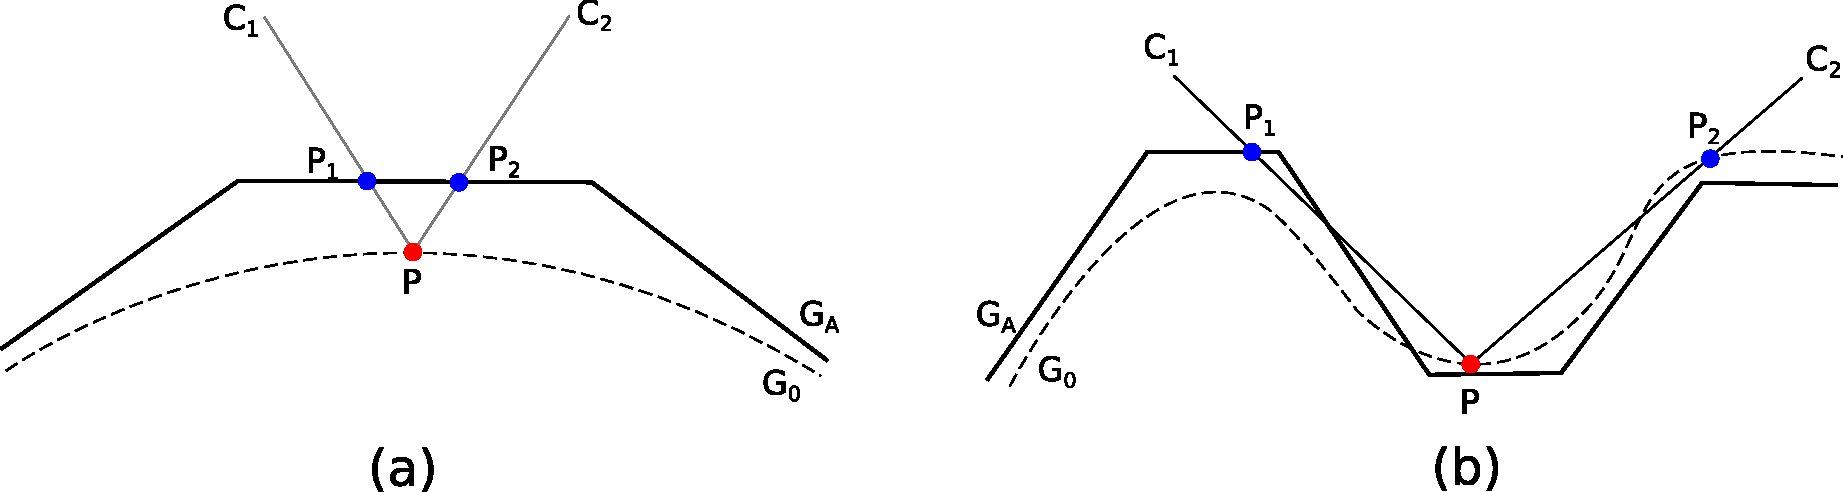
\includegraphics[width=\textwidth]{figures/projection-error}
\caption{(a) chyby v geometrii způsobují chybnou projekci, bod P na původní geometrii je promítnut na body $P_1$ a $P_2$ na aproximované geometrii. (b) chyby ve viditelnosti, bod P je chybně viditelný z kamery $C_2$ a naopak není viditelný z kamery $C_1$.}
\label{fig:projection-error}
\end{center}
\end{figure}

Důležitým prvkem je projekční matice kamery, která nám určuje projekční mapování 3D bodu $(x, y, z)$ do 2D souřadnic $(s, t)$ v $i$-té fotografii  $\textbf{P}_i: (x, y, z) \to (s, t)$, viz sekce \ref{sec:matice-kamery}.  Z promítnuté pozice v obrázku pak můžeme přiřadit 3D bodu barvu $\textbf{I}_i : (s, t) \to (r, g, b)$. Poté libovolný nový pohled $\textbf{I}^V$ z virtuální kamery $V$ můžeme vyjádřit pomocí rovnice \ref{eq:iview} \cite{floating-textures}.

\begin{align}
\label{eq:iview}
\textbf{I}^V(x, y, z, \theta, \phi) = \sum_{i} \textbf{I}_{i}^{V}(x, y, z, \theta, \phi)~\omega_i
\end{align}

\noindent kde

\begin{align}
\label{eq:linear-comb-plen}
\textbf{I}_{i}^{V}(x, y, z, \theta, \phi) &=\textbf{I}_{i}(\textbf{P}_{i}(\textbf{G}_A(x, y, z, \theta, \phi)))\\
\label{eq:linear-weighting}
 \omega_i &= \delta_i(\textbf{G}_A(x, y, z, \theta, \phi)) w_i(x, y, z, \theta, \phi)
\end{align}

\noindent a $\sum_i \omega_i = 1$. Notace $ \textbf{I}_{i}^{V}$ značí vyrenderovaný obrázek z pohledu $V$ promítnutím vstupní fotografie  $\textbf{I}_{i}$ jako textury na povrch  $\textbf{G}_A$. $\delta_i$ určuje viditelnost a je 1, pokud je bod na povrchu $\textbf{G}_A$ viditelný v kameře $i$ a 0 pokud není. $w_i$ je funkce, která určuje váhu kamery $i$ pro každý paprsek. Rovnice \ref{eq:iview} se snaží reprezentovat plenoptickou funkci jako lineární kombinaci promítnutých fotografií.

Zásadní problém spočívá v tom, že $\textbf{G}_A \neq \textbf{G}_0$, tedy již vstupní data vztahu \ref{eq:linear-comb-plen} jsou zatížena chybou (obr. \ref{fig:projection-error}). Problémy přináší také nepřesná kalibrace kamery $\textbf{P}_i$, což způsobuje další nepřesnosti při mapování.

\section{Související práce}
\label{sec:related}

Existuje několik základních metod, jak mapovat fotografie z více pohledů na
model. Jednou z možností je projekce všech fotografií a jejich následné sloučení
pomocí nějakého váženého průměru, jako např. v \cite{Bernardini01}.
Nevýhodou takové metody je zejména vznik artefaktů ve výsledné textuře, často se
projevuje tzv. ghosting, kdy se v textuře objeví několik kopií jednoho obrazce.
Další variantou je vytvoření atlasu textur \cite{Allene08}, kdy každá část
modelu dostane svojí texturu z unikátního pohledu. Tato varianta je využita
např. v \cite{multi-view-tex}. Tento přístup má nevýhodu ve vzniku švů na
okrajích jednotlivých částí textur, které je pak nutné odstraňovat
\cite{seamless-mosaicing}. Kromě artefaktů je u těchto přístupů častým problémem
rozostření některých částí textur. Většina zmiňovaných problémů vzniká kvůli
nepřesné kalibraci fotografií (špatnému odhadu radiální distorze či ohniskové
vzdálenosti) nebo nepřesně rekonstruovaným modelům. Tyto nepřesnosti jsou
obvyklé, i když jsou dnes již algoritmy pro 3D rekonstrukci velmi kvalitní.
Získat velmi přesně kalibrované fotografie je časově náročný proces a někdy i
téměř nerealizovatelný, např. ve venkovních scénách.

V článku \cite{multi-view-tex} jsou uvažovány nepřesně vytvořené modely, které
je nutné otexturovat z původních fotografií, i když na model přesně nepasují.
Navrhují podle modelu upravit původní fotografie a z nich následně vytvořit
atlas textur. Úpravu provádí tak, že ve fotografiích identifikují významné
prvky, které naleznou na vytvořeném modelu a zpětně je promítají do původních
pohledů. Poté deformují všechny fotografie, aby co nejlépe odpovídaly nepřesným
modelům. Touto metodou se nezbaví všech artefaktů, ale omezí jejich výskyt.

Podobný přístup je použitý v \cite{harmonized-texture-mapping}, kde je
popsán způsob, jak dynamicky deformovat několik textur najednou podle 3D modelu
a poté je pomocí vážených faktorů sloučit dohromady na základě pozice virtuální
kamery.

Odlišný přístup je použitý v článku \cite{masked-blending}. Zde řeší texturování
hustých modelů s jednotkami až desítkami milionů trojúhelníků. Pro takto husté
modely nepoužívají textury, ale barvu přiřazují pouze vrcholům, což vzhledem k
počtu vrcholů v modelu poskytuje dostatečné detaily. Základní princip algoritmu
je takový, že model je vykreslen z pohledu jednotlivých kamer a poté jsou
viditelné vrcholy promítnuty zpět do původních fotografií. Pokud je jeden vrchol
vidět na více fotografiích, je použita funkce, která vybere nejvhodnější barvu
pro daný vrchol. Tato funkce používá vážené masky, které jsou vygenerovány pro
každou fotografii a udávají kvalitu jednotlivých pixelů. Pro určení kvality
pixelu je použito několik různých metrik, pro každou fotografii je tedy
vytvořeno více masek (každá maska má rozlišení stejné jako fotografie). Použité
metriky jsou následující:
\begin{itemize}
  \item Úhlová metrika - nejjednodušší metrika, která porovnává směr ke kameře s 
  		normálou plochy. Největší váha je, pokud jsou oba směry stejné.
  \item Hloubková metrika - váha pixelu je větší, pokud je povrch blíže ke 
  		kameře.
  \item Hraniční metrika - tato maska udává, jak daleko je pixel od okrajů 
  		fotografie a silulety v hloubkové mapě. Čím dále je pixel od okrajů, 
  		tím je jeho kvalita lepší.
\end{itemize}
Výsledná váha pixelu je získána vynásobením hodnot v jednotlivých maskách. Tím 
je zaručeno zachování lokálních minim v každé masce, což pomáhá odstraňovat 
pixely, které jsou v libovolné masce považovány za velmi špatné. Výsledná barva 
pro každý vrchol se získá porovnáním masek u všech fotografií, ze kterých je daný 
vrchol viditelný, a následným vybráním nejlepšího pixelu.

Výhoda tohoto způsobu je, že se nejedná o výpočetně složité operace, většina
výpočtů je prováděna nad fotografiemi a není závislá na složitosti modelu. Další
výhodou je možnost určit kvalitu jednotlivých fotografií podle maximální či
průměrné kvality masky. Tím je možné některé nevhodné fotografie automaticky
eliminovat a zrychlit celý proces. Nevýhodou této metody je nutnost hustých
modelů, u modelů s nižším počtem vrcholů by výsledky této metody nebyly příliš
kvalitní. Další problém nastává, pokud je rozlišení fotografií vyšší než
rozlišení modelu (jeden vrchol se mapuje na více pixelů ve fotografiích), to
vyžaduje další zpracování dat a zvyšuje složitost problému.



Všechny tyto algoritmy mají společné to, že z původních pohledů předem vytvoří
texturu či atlas textur spojením všech fotografií, přičemž se snaží
minimalizovat vznik artefaktů nebo případně vzniklé artefakty odstraňovat.
Metoda navržená v této práci se zásadně liší tím, že žádnou takovou texturu
nevytváří, ale pro každý aktuální pohled virtuální kamery vybírá množinu
fotografií z nejvhodnějších pohledů a z této množiny vybírá nejvhodnější texely.
Zásadní nevýhodou tohoto přístupu je velký výpočetní výkon, který je potřeba při
zobrazování modelu. Tuto nevýhodu se snažíme minimalizovat efektivním využitím
GPU.

Tato myšlenka není úplně nová, na podobném principu je založena např. metoda
plovoucích textur \cite{floating-textures}. Tento algoritmus používá adaptivní
nelineární metodu, která opravuje lokální nezarovnání textur vůči 3D modelu. K
tomu určuje optický tok \footnote{v orig. optical flow} mezi promítanými fotografiemi a
příslušné textury kombinuje.

Navrhovaný postup využívá kombinaci lineární interpolace a odhadu optického
toku. Nejprve je provedena projekce fotografií $I_i$ na model z původních
pohledů a scéna je vyrenderována z aktuálního pohledu virtuální kamery $V$. Tím
vzniknou dočasné textury $I_i^V$. Poté je na jednotlivé páry textur $I_i^V$
aplikován odhad optického toku, čímž vzniknou pole $W_{I_i^V \rightarrow
I_j^V}$. Pro více než dvě vstupní fotografie je nutné provést lineární kombinaci
vytvořených polí a sloučit je do výsledné textury $I^v_{Float}$. To je poměrně náročná operace, pro n vstupních fotografií je nutné vytvořit $O(n^2)$ polí. S tím se vyrovnávají v článku tím, že používají pro každý pohled jen 3 nejbližší fotografie. Plovoucí textury porušují epipolární geometrii, což umožňuje texturám kompenzovat nekvalitní kalibraci kamery a nepřesně zrekonstruované 3D modely.

Dále je nutné vypořádat se s vlastním zastíněním částí modelu, což je velmi
běžná situace. K tomu je využita jemná mapa viditelnosti, která pro každý pixel
určuje, zda je z dané kamery viditelný nebo ne. Oproti tradičním postupům, které
obvykle využívají pouze hodnoty 1 a 0 (je nebo není vidět), je zde použita
metoda, která nastavuje hodnotu z intervalu $(0,1)$ pixelům, které jsou blízko
hranic zastínění. Tím jsou odstraněny ostré hrany podél zastíněných částí, které
jsou velmi často nepřesné a snižují výslednou vizuální kvalitu.

Na principu výběru nejlepší fotografie na základě aktuálního pohledu je založená metoda v článku \cite{Debevec96}. Při mapování jedné fotografie navrhují použití image-space stínových map pro řešení viditelnosti, protože to umožňuje efektivní implementaci pomocí z-bufferu. Při mapování více fotografií na model vybírají pro každý pixel vždy takovou fotografii, která se na daný povrch dívá pod nejlepším úhlem. To samozřejmě přináší viditelné švy, protože sousední pixely mohou pocházet z různých fotografií. Toto řeší zjemněním přechodů pomocí váženého průměru, váhu je určena podle rozdílu úhlu aktuálního pohledu a pohledu původní kamery. Dále pro lepší výsledky mají pixely na okraji fotografie menší váhu, čímž se snaží ještě více eliminovat vznik švů.

Dále navrhují jednoduchý algoritmus pro odstranění nežádoucích objektů, které se mohou vyskytovat na zdrojových fotografiích - např. auto či chodci před budovou, kterou chceme otexturovat. Uživatel může ručně vymaskovat tyto objekty předem zvolenou barvou a tyto pixely dostanou při texturování nulovou váhu a budou použita data z jiné fotografie. Pokud nejsou dostupná žádná data, vyplňují vzniklé mezery pomocí syntézy obrazu.

\section{Návrh řešení}

Algoritmus se skládá ze tří základních kroků - projekce fotografií na model, výběr nejlepších fotografií pro pokrytí celého modelu a výběr nejvhodnějšího pixelu z více fotografií pro otexturování fragmentu\footnote{Fragmentem je v textu vždy myšlena plocha na 3D modelu, který odpovídá jednomu výslednému pixelu na obrazovce. Stejně, jako je termín fragment používán v OpenGL.}.

\subsection{Projekce fotografie na model}
\label{sec:matice-kamery}

Mapování jedné fotografie na model můžeme popsat jako projekci $P: (x, y, z) \to (s, t)$, tedy jako projekci 3D bodů modelu do 2D souřadnice ve fotografii, viz obr. \ref{fig:camera-projection}. Nejběžněji se v počítačové grafice a vidění používá perspektivní projekce, která promítá 3D body $p$ na 2D body $x$ vydělením jejich $z$ souřadnicí \cite{Szeliski}. V homogeních souřadnicích má kanonická perspektivní matice \textbf{P}$_0$ jednoduchou formu:
\begin{align}
\label{eq:persp-projection}
x = 
\underbrace{
\begin{bmatrix}
1 & 0 & 0 & 0 \\
0 & 1 & 0 & 0 \\
0 & 0 & 1 & 0 \\
\end{bmatrix}}_\text{\textbf{P}$_0$}
p
\end{align}
\noindent

\begin{figure}[t]
\begin{center}
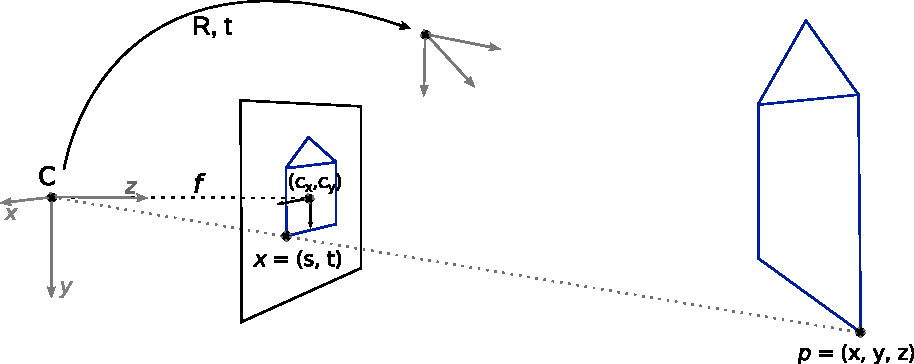
\includegraphics[width=\textwidth]{figures/camera-projection}
\caption{Obrázek znázorňuje situaci při projekci 3D bodu na 2D souřadnice.}
\label{fig:camera-projection}
\end{center}
\end{figure}

Po promítnutí 3D bodu projekční kamerou je nutné transformovat souřadnice na základě vlastností senzoru a orientace kamery vzhledem k počátku souřadnicového systému.  \emph{Kalibrační matice} \textbf{K} transformuje kanonickou perspektivní kameru na standardní projekční kameru \textbf{P}: 
\begin{align}
\label{eq:calibration-matrix}
\textbf{P} = 
\begin{bmatrix}
f & 0 & c_x  \\
0 & f & c_y  \\
0 & 0 & 1  \\
\end{bmatrix}
\cdot
\begin{bmatrix}
1 & 0 & 0 & 0 \\
0 & 1 & 0 & 0 \\
0 & 0 & 1 & 0 \\
\end{bmatrix}
 =\textbf{K}\textbf{P}_0
\end{align}
\noindent
kde $f$ je ohnisková vzdálenost v pixelech a bod $(c_x, c_y)$ je optický střed vyjádřený v pixelech, obr. \ref{fig:camera-projection}. Toto je zjednodušená matice kamery \textbf{K}, která uvažuje senzor kolmý vůči optické ose a stejnou ohniskovou vzdálenost v osách $x$ a $y$ (což je v praxi nejběžnější varianta). Orientaci kamery vůči počátku souřadnicového systému definujeme pomocí $3\times3$ rotační kamery \textbf{R} a vektoru \textbf{t}, čímž získáme výslednou $3\times4$ \emph{matici kamery}:
\begin{align} 
\textbf{P} = \textbf{K}~[~\textbf{R}~|~\textbf{t}~]
\end{align}
\noindent
která provádí mapování bodu $p_w$ v 3D světových souřadnicích do 2D souřadnic $x$ ve fotografii:
\begin{align}
x = \textbf{P}\cdotp p_w
\end{align}
Existuje celá řada algoritmů pro nalezení matice kamery \cite{Hartley2004}, to ale není součástí této práce, kalibrované kamery jsou poskytnuté na vstupu společně s rekonstruovaným modelem a fotografiemi.

Při mapování fotografie na model je nutné brát v úvahu, že některé části modelu mohou být vzhledem ke kameře zastíněné a nemohou být z dané kamery správně otexturovány. Toto se nejčastěji řeší pomocí stínových map \cite{Stamminger2002}, které se předem vytvoří pro každou kameru. Aby byla tato metoda kvalitní, musí mít stínové mapy dostatečné rozlišení.  Vzhledem k tomu, že aplikace bude využívat až stovky různých kamer, bylo by použití této metody paměťově velmi náročné.

Další možností je použít algoritmus vrhání paprsků, kdy se z kamery vrhají na scénu paprsky a podle zásahů s modelem se určí, které fragmenty jsou z kamery viditelné. Tato metoda také není příliš vhodná, protože aplikace bude v reálném čase využívat až desítky různých kamer zároveň a vrhání dostatečného množství paprsků z každé kamery by bylo výpočetně příliš náročné. Proto se jako nejlepší varianta se jeví využít jednodušší algoritmus, který spoléhá na seřazení kamer podle podobnosti se směrem virtuální kamery. Kvůli velkému množství vstupních kamer se dá očekávat, že pro většinu možných pohledů virtuální kamery bude existovat kamera s velmi podobným pohledem. Pro takovou kameru bude existovat jen velmi malé množství oblastí, které budou z kamery zastíněné, ale z virtuální kamery budou viditelné. Při texturování se kamery seřadí od ``nejlepší'' a každá kamera bude využita k otexturování oblasti, která ještě není pokrytá předchozí kamerou. Tím se výrazně omezí oblasti, které jsou otexturovány zastíněnou kamerou, ale zároveň jsou viditelné z virtuální kamery. K tomuto pravidlu je navíc zaveden práh, který určuje minimální úhel mezi směrem kamery a normálou plochy, pro který může být daná plocha kamerou otexturována. 


\subsection{Výběr vhodných fotografií pro otexturování modelu}
\label{sec:photo-choosing}

Téměř vždy nestačí k otexturování aktuálního pohledu pouze jedna fotografie. Proto je potřeba použít více fotografií pro vyrenderování modelu z nového pohledu. Na obrázku \ref{fig:dum-1} je zobrazen model s jednou a se dvěma namapovanými fotografiemi.  Při mapování více fotografií zároveň je nutné vyřešit dva základní problémy - které fotografie budou vybrány a jak bude fragment otexturován, pokud je jeho polohu možné promítnout do více kamer.

\begin{figure}[bh]
\begin{center}
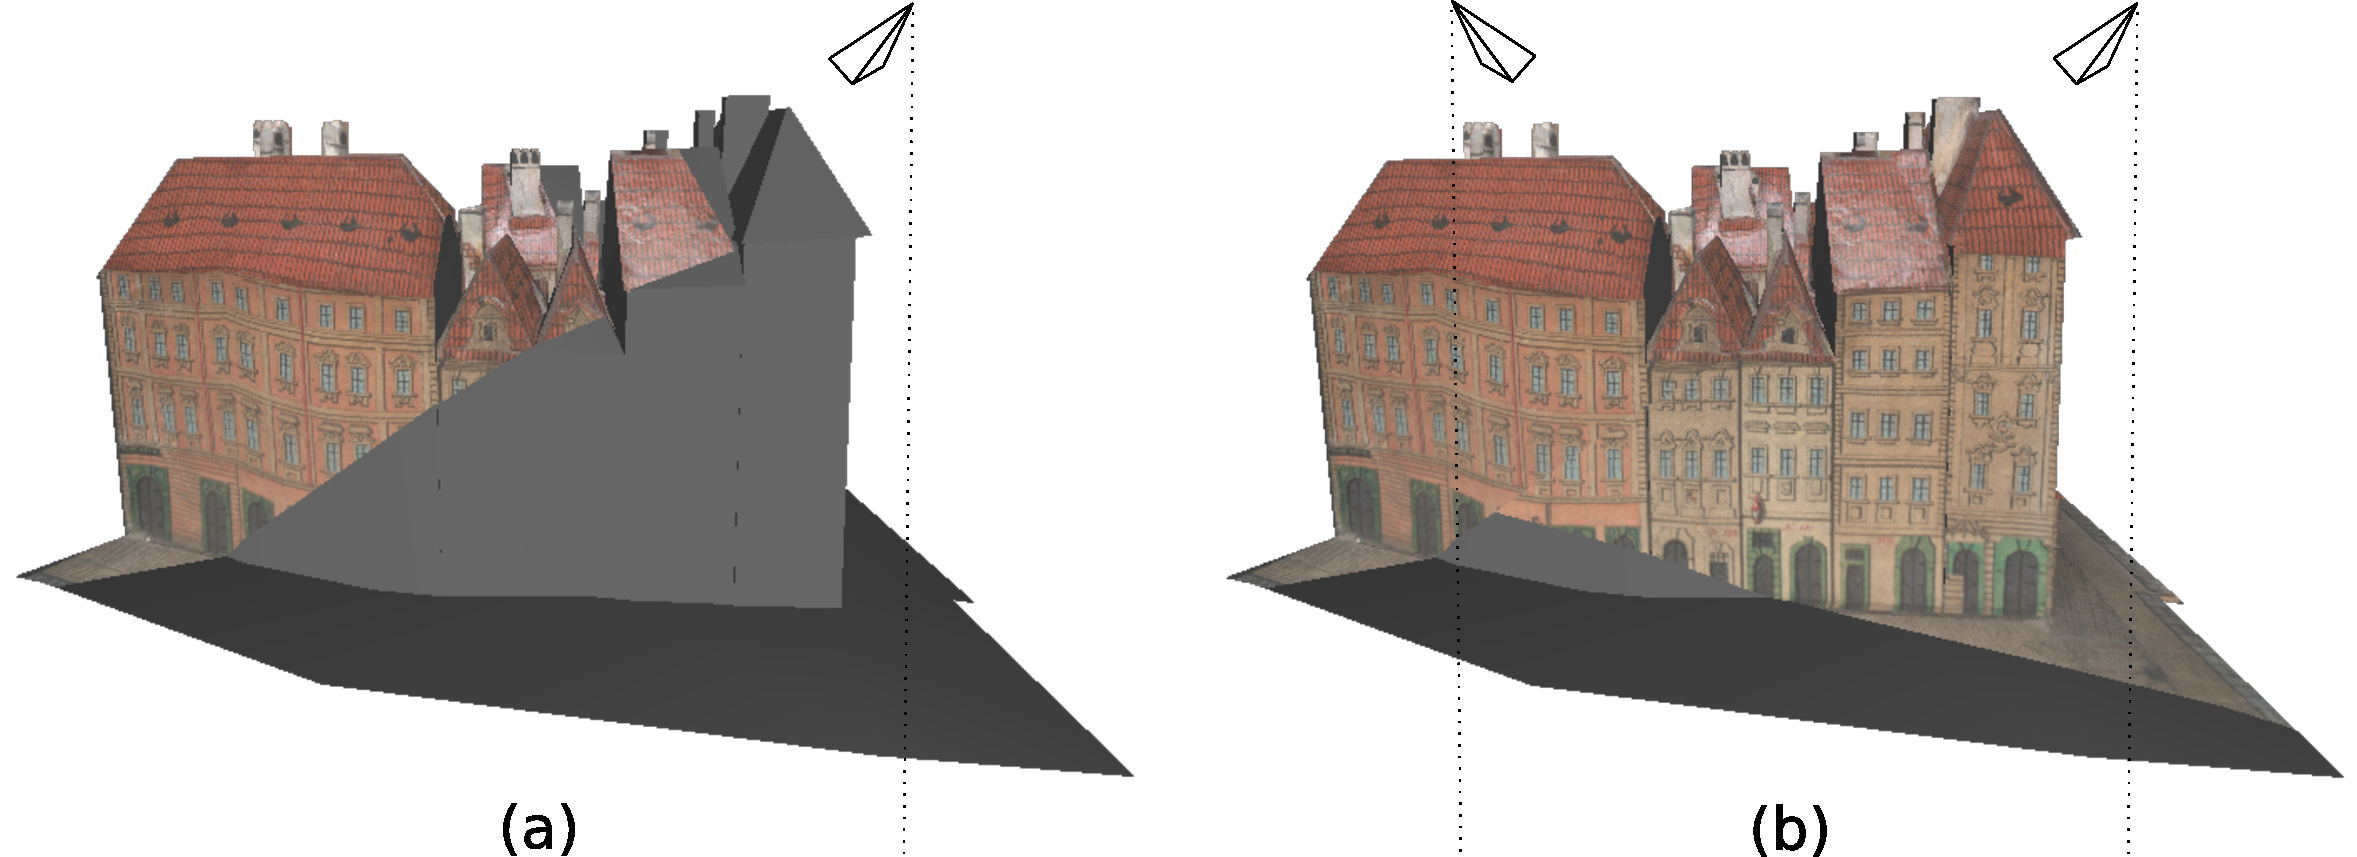
\includegraphics[width=\textwidth]{figures/dum-1}
\caption{Projekce jedné (a) a dvou (b) fotografií na 3D model. Pozice kamer jsou pouze ilustrační.}
\label{fig:dum-1}
\end{center}
\end{figure}

Výběr fotografií je je prováděn na základě shody aktuálního pohledu virtuální kamery s pohledy vstupních kamer. Pro porovnání je nutné určit, kterým směrem jsou kamery natočeny.  U vstupních kamer jde tento směr zjistit přímo z matice kamery, ale nemusí to být vždy výhodné. Pokud se kamera nedívá přímo na objekt (optická osa neprochází objektem), může být směr kamery poměrně zavádějící. Proto navrhujeme algoritmus, který tento směr koriguje na základě viditelné části modelu na fotografii. Tato metoda funguje tak, že se vrcholy rekonstruovaného modelu promítnou do fotografie, body ležící mimo fotografii se zahodí. Poté je nalezena konvexní obálka \cite{Andrew79} promítnutých bodů, která přibližně ohraničuje oblast modelu zobrazenou na fotografii, viz obr. \ref{fig:convex-hull}. Z bodů ležících na konvexní obálce se spočítá centroid a nalezne se směrový vektor ze středu kamery procházející centroidem. Nalezený vektor se použije jako výsledný směr pohledu kamery. Algoritmus není příliš náročný, promítnutí $n$ vrcholů do obrázku je provedeno se složitostí $\Theta(n)$, konvexní obálku ve 2D lze nalézt se složitostí $0(n~log(n))$. Během tohoto algoritmu je zároveň vypočtena plocha konvexní obálky (plocha konvexního polygonu s vrcholy v bodech konvexní obálky). Tato plocha je později při texturování fragmentů zahrnuta do výpočtu váhy fotografie, viz sekce \ref{sec:fragment-texturing}.

\begin{figure}[th]
\begin{center}
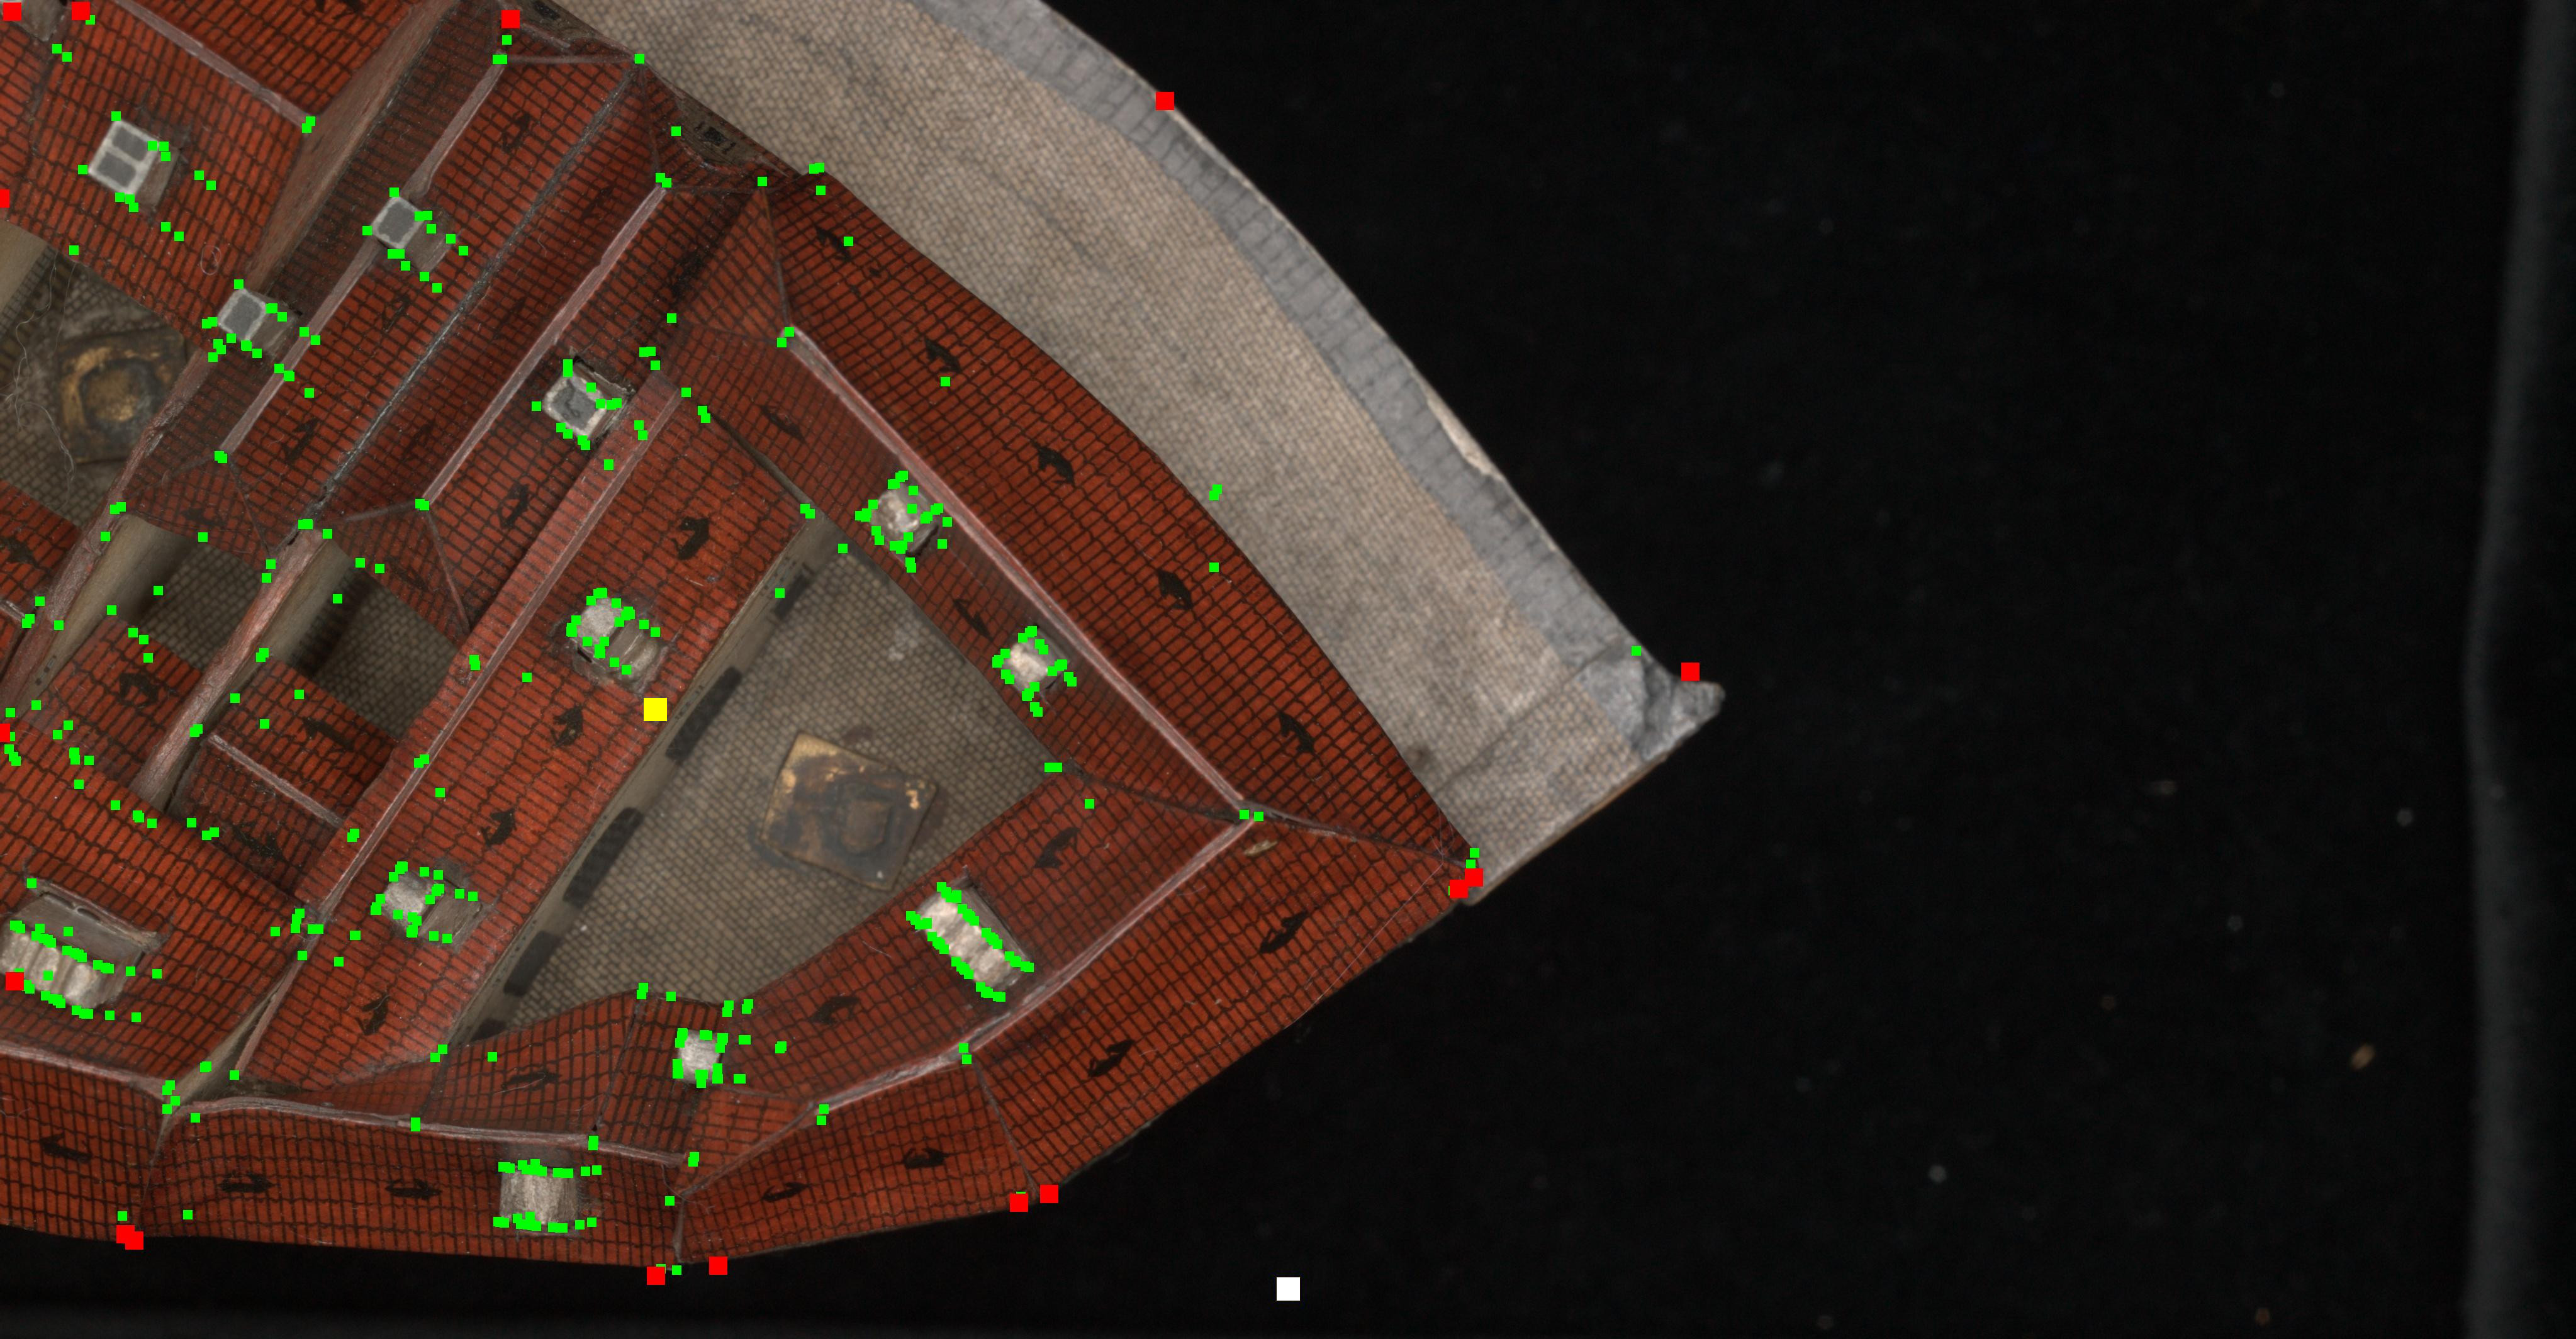
\includegraphics[width=\textwidth]{figures/0-0270_1020_110_09_00_000_098345e}
\caption{Výřez horní poloviny fotografie použité k texturování. Bílý bod označuje průnik optické osy s obrázkem, žlutý bod označuje vypočtený centroid. Ostatní body jsou vrcholy 3D modelu promítnuté do obrázku, červeně zvýrazněné vrcholy leží na konvexní obálce.}
\label{fig:convex-hull}
\end{center}
\end{figure}
 
Podobná situace nastává při určování směru virtuální kamery.  Pokud se díváme zvenku na model a otáčíme virtuální kamerou, vidíme model stále ze stejného směru a chceme, aby byl otexturován stejně. Proto není vhodné použít přímo směr, kterým se dívá virtuální kamera, ale spíše spojnici mezi pozicí kamery a modelem. Pro určení pozice modelu je použit centroid všech vrcholů. Odlišná situace nastává, pokud se virtuální kamera nachází uvnitř modelu. V tomto případě naopak musíme brát v úvahu přímo směr pohledu virtuální kamery, protože při otočení kamery vidíme jinou část modelu. K jednoduchému určení, zda je kamera uvnitř nebo vně modelu, je možné použít osově zarovnaný ohraničující kvádr (AABB).


Po vypočtení směru pohledu vybereme nejlepší fotografie porovnáním se směry všech vstupních kamer. Počet fotografií potřebných k otexturování je závislý na složitosti scény a i na samotných fotografiích, proto se tato hodnota nenastavuje automaticky, ale uživatel jí musí zadat na vstupu.

Pro otexturování modelu často nestačí vybrat pouze fotografie, které nejlépe odpovídají aktuálnímu pohledu. Takové fotografie dobře pokryjí plochy, které jsou na aktuální pohled přibližně kolmé. Oproti tomu velmi špatně pokryjí plochy, které jsou téměř paralelní se směrem aktuálního pohledu, ale zároveň jsou ještě dobře viditelné, obr. \ref{fig:faces-no-tex} (a). K určení takových ploch je nutné zavést práh, který definuje maximální úhel mezi normálou plochy a směrem kamery, kdy je ještě možné plochu kvalitně otexturovat. Během testování se ukázalo vhodné použít práh přibližně $70^{\circ}$. 


\begin{figure}[th]
\begin{center}
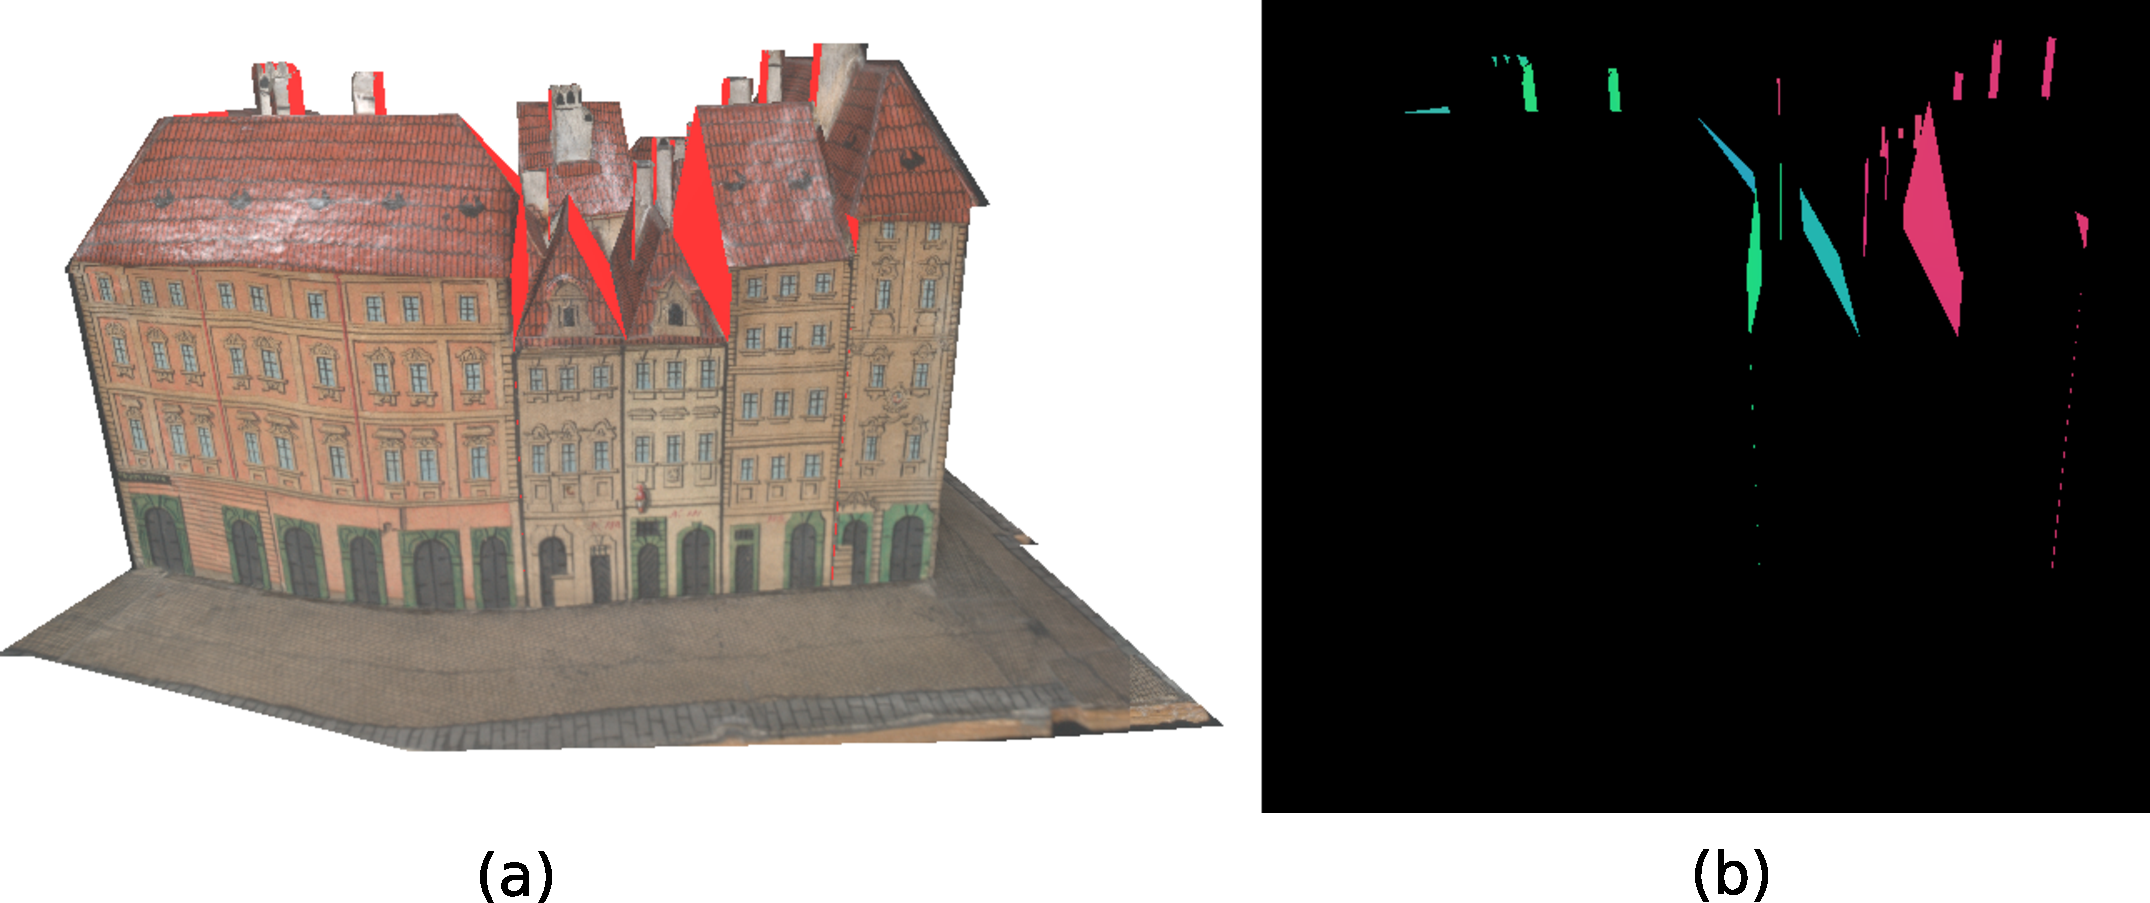
\includegraphics[width=\textwidth]{figures/faces-no-tex}
\caption{(a) Model otexturovaný šesti fotografiemi z kamer, které nejlépe odpovídají pohledu virtuální kamery. Červeně jsou zvýrazněny plochy, které nejde z kamer kvalitně otexturovat. (b) Vyrenderovaná textura s uloženými normálami v prvním průchodu algoritmu ze stejného pohleduj jaklo (a).}
\label{fig:faces-no-tex}
\end{center}
\end{figure}

K efektivnímu nalezení těchto ploch navrhujeme dvou průchodový algoritmus. Nejprve se vybere daný počet fotografií, které nejlépe odpovídají aktuálnímu pohledu. Poté se v prvním průchodu model vykreslí a zjistí se, které plochy je s daným prahem možné z vybraných fotografií otexturovat. Pokud fragment není možné pokrýt žádnou fotografií, vykreslí se do textury aktuální normála. V prvním průchodu tedy vznikne textura, která obsahuje normály ploch, které je nutné pokrýt, obr. \ref{fig:faces-no-tex} (b). Poté je provedeno klastrování těchto normál a jsou určeny nejvýznamnější směry. Tento přístup je vhodný, protože klastrování jde efektivně provést na GPU bez nutnosti přenosu velkého množství dat mezi GPU a CPU. Poté se vyberou nové fotografie, které nejlépe odpovídají nalezeným směrům (kamery, jejichž směr pohledu je opačný k nalezeným normálám). V druhém průchodu se poté provede výsledný rendering. 

\subsection{Texturování z více fotografií}
\label{sec:fragment-texturing}
Během renderingu je nutné vyřešit, jak budou otexturovány fragmenty, pro které je možné použít data z více fotografií. Princip je velmi podobný, jako při výběru fotografií, ale snahou při texturování je také omezení vzniku švů a omezení chybného otexturování zastíněných oblastí. Během texturování se již používají pouze fotografie, které byly vybrány v předchozím kroku.

Pro každou fotografii je vypočtena váha, fotografie s nejvyšší váhou je použita pro otexturování. Jeden fragment je otexturován pouze z jedné fotografie, není použito žádné vážené míchání barev z více fotografií. To vede k tomu, že dva sousední pixely mohou být vybrány z různých fotografií a tím mohou vznikat viditelné švy. Vážené míchání barev, jako např. v \cite{Debevec96} vede k rozmazání textur a na testovacích datech k vizuálně horšímu výsledku. 

Váha $w_i$ $i$-té fotografie je složena z několika faktorů. V úvahu je brána shoda směru kamery $d_c$ se směrem virtuální kamery $d_v$, stejně jako při výběru fotografií. Dále se uvažuje úhel mezi směrem kamery a normálou plochy $N_f$. Tím se preferují kamery s co nejvíce kolmým pohledem na danou plochu a zároveň je pravděpodobnější, že celá plocha bude otexturována z jedné fotografie. Nakonec je do výpočtu zahrnuta  velikost plochy $s_i$, kterou na fotografii zabírá model, viz výpočet konvexní obálky v sekci \ref{sec:photo-choosing}. Celkový výpočet váhy shrnuje následující rovnice:

\begin{align}
\label{eq:weight-scheme}
w_i &= dot(d_v, d_c) \times \left(\frac{1 + dot(-N_f, d_c)}{1 - cos(\alpha)} + 1\right) \times s_i \times \delta(i)\\
\delta(i) &= \left\{
  \begin{array}{l l}
    1 & \quad \text{pokud~$\exists P_i:(x, y, z) \to (s, t)$}\\
    0 & \quad \text{v opačném případě}
  \end{array} \right.
\end{align}

\noindent kde $dot$ značí skalární součin dvou vektorů a $\alpha$ je limitní úhel, který určuje, zda je plochu možné z dané kamery otexturovat.

Musíme brát v úvahu, že máme dvě rozdílné množiny fotografií. Nejprve jsme vybrali fotografie, které nejlépe odpovídají aktuálnímu pohledu. Poté jsme nalezli doplňující fotografie, které pokryjí zbývající plochy. Proto musí rendering probíhat ve dvou částech. Nejprve se aplikuje původní množina fotografií. Až poté se použijí doplňující fotografie, které mohou otexturovat pouze fragmenty, které se nepodařilo otexturovat v první části. Tímto se jednak preferují fotografie blízké aktuálnímu pohledu a zároveň se omezí  případné chyby, kdy by doplňující fotografie mohly otexturovat plochy, které jsou z jejich pohledu zastíněné. K tomu i tak může dojít, ale pouze ve velmi omezených částech výsledného renderu.




\chapter{Implementace}

\chapter{Testování}

\chapter{Závěr}


\renewcommand\refname{Zdroje}
\bibliographystyle{alpha}
\def\CS{$\cal C\kern-0.1667em\lower.5ex\hbox{$\cal S$}\kern-0.075em $}
\bibliography{zdroje}


\appendix


\chapter{Seznam použitých zkratek}

\begin{description}
\item[2D] Two-Dimensional
\item[ABN] Abstract Boolean Networks
\item[ASIC] Application-Specific Integrated Circuit
\end{description}
\vdots

%*****************************************************************************
\chapter{Instalační a uživatelská příručka}

%*****************************************************************************
\chapter{Obsah přiloženého CD}


\end{document}
